\chapter{Writing a thesis in LaTeX}
A LaTeX document class has been developed, which follows the guidelines
described in \cite{kulemtgl}. The usage of this class is described in
\Cref{cha:kulemt}. The result can be customized and adapted to the masters'
guidelines with the class options. Additional functionality is available
through numerous LaTeX packages (cf.\ \Sref{sec:packages}). Just make sure
that the final result still conforms to the guidelines.

\Aref{app:template} contains a typical LaTeX template. Since each chapter
is a logical unit and since it's usually several pages long, chapters
should be put in independent files. They are called from the main file
using the LaTeX \cs{include} mechanism. The bibliography is a special case.
It is handled in \Sref{sec:bibtex}.

If you are not (yet) familiar with LaTeX, you should first have a look at the
documentation of the TeX Users Group on \url{http://tug.org/begin.html}.
It also contains a list of on-line tutorials and manuals. The most popular
(not so) short introduction to LaTeX is probably \cite{lshort}.
\Sref{sec:packages} contains some extra information on how to install LaTeX
packages. It also lists some typically useful packages.

\section{Using extra LaTeX packages}
\label{sec:packages}
Most of the packages mentioned in this document are present a standard
LaTeX installation, with the exception of the \pkg{kulemt} package. Apart
from this \pkg{kulemt} package, only a few packages are required. An
overview is given in \tref{tab:reqpack}.
\begin{table}[t]
  \caption[Packages used by \cls{kulemt} which may not be present in your
    LaTeX installation.]{Packages used by \cls{kulemt} which may not be
    present in your LaTeX installation. If a package is desirable but not
    required, it is used when available and ignored otherwise.}
  \label{tab:reqpack} 
  \centering
  \newcommand*\citepkg[1]{\pkg{#1}&\cite{pkg:#1}}
  \begin{tabular}{@{}l@{\space}ll@{}}
    \toprule
    Package           & & Remarks \\
    \midrule
    \citepkg{memoir}    & Required; at least version 1.61 (2004-04-05) \\
    \citepkg{microtype} & Desirable unless option \opt{nomicrotype} is used\\
    \pkg{lmodern} (\pkg{lm}) & \cite{pkg:lmodern}
                        & Desirable; required if \opt{font=lm} is used \\
    \citepkg{fourier}   & Only required if \opt{font=utopia} is used \\
    \bottomrule
  \end{tabular}
\end{table}

When you want to install a package, you can follow the instructions found
in the TeX-FAQ\,\cite{texfaq} under the heading ``Installing (La)TeX
files''. If you only can or want to install packages for your personal use,
make sure you read ``Private installations of files''.

The installation of the document class \cls{kulemt} is done in the same way
as the installation of any other package. The only difference is the fact
that its source is not available from \acro{CTAN} but from a local ftp
server\,\cite{pkg:kulemt}.

Apart from the required packages, a lot of packages are available from
\acro{CTAN}\,\cite{CTAN}\footnote{An alphabetic and a topical index is
  provided by the TeX Catalogue\,\cite{texcatalogue}.}, which can help you
to make your text easier to understand or more impressive. Many of them are
installed by default in a traditional LaTeX installation. Some typical
examples are given in \tref{tab:otherpack}.
\begin{table}
  \caption{Packages which can be useful to extend the \cls{kulemt} class.}
  \label{tab:otherpack}
  \centering
  \renewcommand*\thefootnote{\fnsymbol{footnote}}
  \begin{tabular}{@{}ll@{}}
    \toprule
    Package        & Description \\
    \midrule
    \pkg{hyperref} & Provide hyperlinks in \PDF\ files \\
    \pkg{amsmath}  & Extra mathematical constructs \\
    \pkg{amssymb}  & Extra mathematical symbols\footnotemark[1]
                         (only for the fonts \opt{cm} \& \opt{lm}) \\
    \pkg{cite}     & Better references \\
    \pkg{babelbib} & Multilingual or non-English bibliographies \\
    \pkg{flafter}\footnotemark[2]
                   & Put figures \& tables always after their definition \\
    \pkg{rotating} & Rotating material, e.g., figures en tables \\
    \pkg{listings} & Typeset programming code \\
    \pkg{nomencl}  & Produce lists of symbols (nomenclature) \\
    \pkg{pgf}      & Create graphics in LaTeX \\
    \pkg{siunitx}  & Consistent use of SI units \\
    \pkg{textcomp}\footnotemark[2]
                   & Extra text symbols\footnotemark[1]
                         (e.g., \cs{texteuro} = \texteuro)\\
    \bottomrule \addlinespace
    \multicolumn2{l}{\footnotemark[1] \footnotesize
      A list of all kind of symbols is found in \cite{symbols}.} \\
    \multicolumn2{l}{\footnotemark[2] \footnotesize
      Information on this package is found in the TeX-FAQ\,\cite{texfaq}.} \\
  \end{tabular}
\end{table}
The loading order can be important for some combination of packages:
packages, which extend or redefine commands of other packages, must be
loaded last.

If you are making a \PDF\ file for on-line distribution, the use of the
\pkg{hyperref} package\,\cite{pkg:hyperref} is a must. It not only
automatically generates the bookmarks, but it also gives you all the
linking facilities required in modern on-line documents\,\footnote{This
  document uses as \pkg{hyperref} options: ``\opt{pdfusetitle,
    colorlinks, \let\meta\relax filecolor=\marg{\oarg{rgb}\marg{0,0,1}},
    urlcolor=\marg{\oarg{rgb}\marg{0,0,1}},
    citecolor=\marg{\oarg{rgb}\marg{0,0,0.4}},
    linkcolor=\marg{\oarg{rgb}\marg{0,0,0.4}}}''.}.

The \pkg{microtype} package\,\cite{pkg:microtype} enhances the typographic
quality of the text. Therefore the \cls{kulemt} class uses it by default.
The most important enhancements provided by the package are character
protrusion and font expansion. Character protrusion lets some characters
enter the margin to provide optical margins. Font expansion creates fonts
which are a little bit narrower or wider. It generates more equal interword
spacing and it provides also more flexibility to avoid hyphenation. Both
effects are illustrated in \fref{fig:microtype}.
\begin{figure}
  \centering
  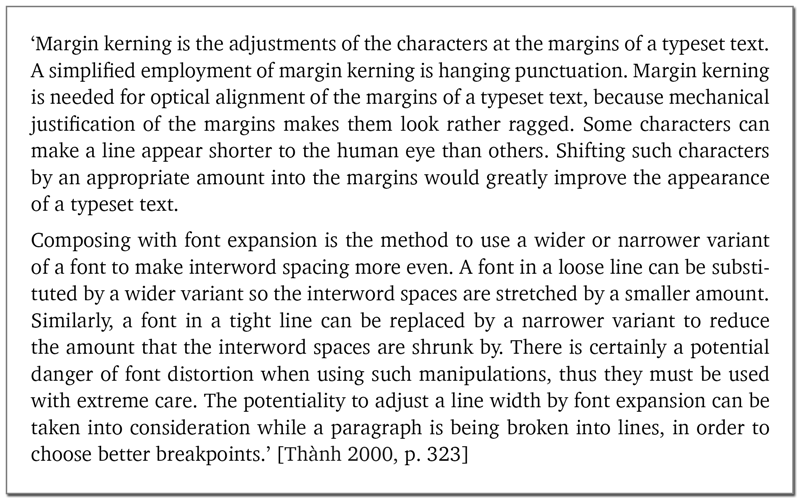
\includegraphics[width=\columnwidth]{expfprof.png}%
  \subcaption{Text typeset without using \pkg{microtype}.}
  \par\bigskip
  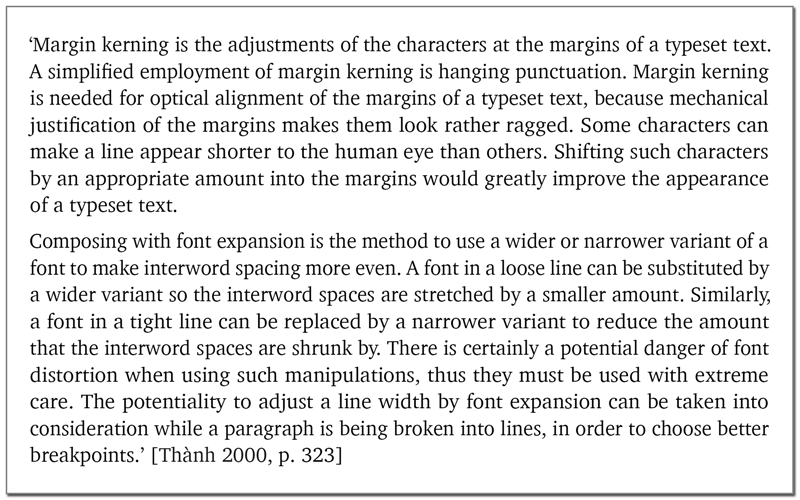
\includegraphics[width=\columnwidth]{exptprot.png}%
  \subcaption{The same text typeset using \pkg{microtype} (character
    protrusion \& font expansion).}
  \caption[The effect of using the \pkg{microtype} package.]{The effect of
    using the \pkg{microtype} package. These examples are borrowed from the
    \pkg{microtype} manual.}
  \label{fig:microtype}
\end{figure}

%\enlargethispage{3pt}
The document class \cls{memoir} includes or emulates a lot of packages. The
exact list of packages included or emulated in \cls{memoir} can always be
found in the log file after a LaTeX run. The emulation not always
corresponds to the latest version of the package, but the main
functionality is usually present. So before installing a new package, first
check the \cls{memoir} manual to see if the functionality is not already
present in the document class.

Since the document class \cls{kulemt} is based on \cls{memoir} it also
includes all packages included or emulated by \cls{memoir\,\footnote{The
    \cls{memoir} class dated 2005-09-25 emulates the packages
    \pkg{abstract}, \pkg{appendix}, \pkg{array}, \pkg{booktabs},
    \pkg{ccaption}, \pkg{chngcntr}, \pkg{chngpage}, \pkg{crop},
    \pkg{dcolumn}, \pkg{delarray}, \pkg{enumerate}, \pkg{epigraph},
    \pkg{framed}, \pkg{ifmtarg}, \pkg{ifpdf}, \pkg{index}, \pkg{makeidx},
    \pkg{moreverb}, \pkg{needspace}, \pkg{newfile}, \pkg{nextpage},
    \pkg{patchcmd}, \pkg{shortvrb}, \pkg{showidx}, \pkg{tabularx},
    \pkg{titleref}, \pkg{titling}, \pkg{tocbibind}, \pkg{tocloft},
    \pkg{verbatim}, and \pkg{verse}. The version dated 2009-11-17 adds the
    packages \pkg{changepage}, \pkg{ifetex}, \pkg{ifluatex}, \pkg{ifxetex},
    \pkg{mparhack}, \pkg{pagenote}, \pkg{parskip}, and \pkg{setspace}.}}.
It further includes some standard packages (\pkg{babel}, \pkg{color},
\pkg{graphicx}, and \pkg{keyval}) as well as the packages mentioned in
\tref{tab:reqpack}.

\section{Using BibTeX for the bibliography}
\label{sec:bibtex}
The bibliography can be input as a list in the text, using the
\env{thebibliography} environment. An alternative way to generate a
bibliography is with the help of the BibTeX program, which is always
included in a LaTeX distribution. More information on building a
bibliography can be found in \cite{tamethebeast} and \cite{btxfaq}.

The bibliographic data is stored in one or more bibliographic files (files
with extension ``\file{.bib}''). For some disciplines existing data files
can be used. They are declared with the \cs{bibliography} command. A
personal data file can also be used \cite[part~3]{tamethebeast}. It's no
problem if the data files contain unneeded items because only the
referenced items will be used.

The actual layout and formatting is determined by the bibliography style.
This style is declared by the \cs{bibliographystyle} command, which refers
to a file with extension ``\file{.bst}''. The master guidelines or the
thesis supervisor determine which bibliography style to use. If none is
specified, you can choose whichever you find most suited for your text.

Some bibliography styles needs additional LaTeX commands for proper
operation. These commands are defined in an accompanying LaTeX style file,
which must be required with \cs{usepackage}. An example is
\pkg{IEEEtrantools}, which defines the command \cs{bstctlcite} to control
the parameters of the \pkg{IEEEtran} bibliography style\footnote{Both the
  \pkg{IEEEtran} bibliography style and the \pkg{IEEEtrantools} style file
  are part of the \pkg{IEEEtran} package\,\cite{pkg:IEEEtran}.}, which is
used in this document. This bibliography style can be used to typeset a
bibliography according to the rules of IEEE\@.

LaTeX packages can also be used to change the formatting of the citations
in text. A popular one is the \pkg{natbib} package \cite{pkg:natbib}. It is
compatible with many bibliography styles and it allows both author-year and
numerical citations.

\section{Using \file{latex} or \file{pdflatex}?}
\label{sec:engine}

The ways to compile a LaTeX file are shown in \fref{fig:compile}.
\begin{figure}
  \newcommand*\pnode[2][]{\path (#2) node[rectangle, draw, thick,
    minimum width=20\unitlength, minimum height=10\unitlength,#1]}
  \newcommand*\fnode[2][]{%
    \draw[thick,#1] (#2) +(-5,5) -- +(5,5) --
      +(5,-5) .. controls +(3,-3)  and +(2,1)  .. % (-2,2)  & (2,1)
      +(0,-5) .. controls +(-2,-6) and +(2,-2) .. % (-2,-1) & (2,-2)
      +(-5,-5) -- cycle;
    \path (#2) node[rectangle, minimum width=10\unitlength,
                    minimum height=10\unitlength]}
  \setlength\unitlength{1mm}
  \centering
  \begin{tikzpicture}[x=\unitlength, y=\unitlength, semithick, >=stealth']
    \ttfamily\small
    %% program nodes
    \pnode{30,17}(pltx){latex};
    \pnode[dashed]{80,10}(pbtx){bibtex};
    \pnode{80,25}(pdps){dvips};
    \pnode[dotted]{80,40}(pp2p){ps2pdf};
    %% file nodes
    \fnode{  5,25}(ftex){.tex};
    \fnode{ 55,25}(fdvi){.dvi};
    \fnode{102,25}(fps){.ps};
    \fnode{ 55,10}(faux){.aux};
    \fnode[dashed]{102,10}(fbbl){.bbl};
    \fnode[dotted]{102,40}(fpdf){.pdf};
    %% arrows
    \draw[->] (ftex.east) -- ++(5,0) |- ($(pltx.west)+(0,2.5)$);
    \draw[->] ($(pltx.east)+(0,2)$)  -- ++(5,0) |- (fdvi.west);
    \draw[->] (fdvi) -- (pdps);
    \draw[->] (pdps) -- (fps);
    \draw[->] ($(pltx.east)+(0,-2)$) -- ++(5,0) |- (faux.west);
    \draw[->] (faux.east) -- ++(4,0) |- (15,2)
              |- ($(pltx.west)+(0,-2.5)$);
    \draw[dashed,->] ($(faux.east)+(4,0)$)  -- (pbtx);
    \draw[dashed,->] (pbtx) -- (fbbl);
    \draw[dashed,->] (fbbl.east) -- ++(5,0) |- (12,0) |- (pltx.west);
    \draw[dotted,->] (fps.east) -- ++(5,0) |- (65,32) |- (pp2p.west);
    \draw[dotted,->] (pp2p) -- (fpdf);
  \end{tikzpicture}\medskip
  \subcaption{Converting a LaTeX file to PostScript (or \PDF\ with the dotted
    part added) using \file{latex}.\label{fig:latex}}
  \par\bigskip\bigskip
  \begin{tikzpicture}[x=\unitlength, y=\unitlength, semithick, >=stealth']
    \ttfamily\small
    %% program nodes
    \pnode{30,17}(pltx){pdflatex};
    \pnode[dashed]{80,10}(pbtx){bibtex};
    %% file nodes
    \fnode{ 5,25}(ftex){.tex};
    \fnode{55,25}(fpdf){.pdf};
    \fnode{55,10}(faux){.aux};
    \fnode[dashed]{102,10}(fbbl){.bbl};
    %% arrows
    \draw[->] (ftex.east) -- ++(5,0) |- ($(pltx.west)+(0,2.5)$);
    \draw[->] ($(pltx.east)+(0,2)$)  -- ++(5,0) |- (fpdf.west);
    \draw[->] ($(pltx.east)+(0,-2)$) -- ++(5,0) |- (faux.west);
    \draw[->] (faux.east) -- ++(4,0) |- (15,2)
              |- ($(pltx.west)+(0,-2.5)$);
    \draw[dashed,->] ($(faux.east)+(4,0)$)  -- (pbtx);
    \draw[dashed,->] (pbtx) -- (fbbl);
    \draw[dashed,->] (fbbl.east) -- ++(5,0) |- (12,0) |- (pltx.west);
  \end{tikzpicture}\medskip
  \subcaption{Converting a LaTeX file to \PDF\ using \file{pdflatex}.%
    \label{fig:pdflatex}}
  \par\medskip
  \caption[Steps to compile a LaTeX file]{Steps to compile a LaTeX file.
    The dashed part is needed only if a BibTeX bibliography is used.
    As long as the \file{.aux} file (or the \file{.bbl} file) changes,
    (\file{pdf})\file{latex} must be invoked.}\label{fig:compile}
\end{figure}
The traditional way uses the \file{latex} program (\fref{fig:latex}). It
outputs the typeset document to a \file{.dvi} file, which is rather TeX
specific. So usually this is converted to a PostScript file using
\file{dvips} or a \PDF\ file using \file{dvips}~+~\file{ps2pdf} or
\file{dvipdfm}.

Several iterations of \file{latex} may be required. Each time the contents
of an auxiliary file (such as \file{.aux} or \file{.bbl}) changes,
\file{latex} must be invoked. This often means three iterations. The first
invocation of \file{latex} generates a list of internal references and of
referenced bibliography items in the \file{.aux} file. The latter is used
by \file{bibtex} to produce the bibliography data in the \file{.bbl} file.
A second iteration uses the bibliography data and the values from the
references from the \file{.aux} file to generate the final content
containing the table of contents and the bibliography. Because this may
introduce new content, labelled items may shift. This requires an additional
iteration of \file{latex} to get the changed references right. The exact
number  of iterations depends on how much references change from one
version of the \file{.tex} file to the next version. If you use an
intelligent editor, such as Emacs with AUCTeX, you needn't guess
yourself: the editor will tell you when an extra iteration is needed.

If you want a \PDF\ file as a result\,\footnote{Every master thesis must
  also be submitted electronically in \PDF!}, it's easier to use
\file{pdflatex} than \file{latex}, as illustrated in \fref{fig:pdflatex}.
But \file{pdflatex} has other advantages too. It uses the pdfTeX engine,
which is an enhanced implementation of the TeX engine used by \file{latex}.
Therefore more advanced features, such as breaking hyperlinks
(\pkg{hyperref} package) or font expansion (\pkg{microtype} package), are
only possible with the pdfTeX engine. Additionally, the pdfTeX engine can
directly include images in the \acro{JPEG} or \acro{PNG} file format as
well as other \PDF\ files. Simple PostScript (e.g., as generated by
MetaPost) can also be included but general \acro{EPS} (Encapsulated
Postscript) not. You'll have to convert the latter to \PDF\ with the
\file{epstopdf} program.

Is there any reason to use \file{latex}? The most important reason is the
fact that your text depends on packages which work only with PostScript
output, such as \pkg{psfrag} or all kind of PSTricks packages. But often
valid or even better replacements exist, such as the \pkg{pgf}
package\,\cite{pkg:pgf}. Conversion tools may also be available (e.g., the
\pkg{pst-pdf} package).
Another valid reason to stick to \file{latex} is the fact that your
thesis supervisor wants you to use it. In this case I hope you can educate
him/her to upgrade to a newer way of working.

You even have more choices than \file{latex} and \file{pdflatex}. A modern
installation also provides \file{xelatex} and \file{lualatex}. Unless you
know what you're doing, I wouldn't recommend them. Furthermore the LaTeX
document class \cls{kulemt} has never been tested with one of them. So it's
very likely you run into problems if you use them.

A final word of advice: don't switch between engines gratuitously. To avoid
errors and text drifting to other places, always use either \file{latex} or
\file{pdflatex}.


%%% Local Variables: 
%%% mode: latex
%%% TeX-master: "kulemt"
%%% End: 
